%
% The first command in your LaTeX source must be the \documentclass command.
\documentclass[sigconf]{acmart}

%
% defining the \BibTeX command - from Oren Patashnik's original BibTeX documentation.
\def\BibTeX{{\rm B\kern-.05em{\sc i\kern-.025em b}\kern-.08emT\kern-.1667em\lower.7ex\hbox{E}\kern-.125emX}}
    
% Rights management information. 
% This information is sent to you when you complete the rights form.
% These commands have SAMPLE values in them; it is your responsibility as an author to replace
% the commands and values with those provided to you when you complete the rights form.
%
% These commands are for a PROCEEDINGS abstract or paper.
\copyrightyear{2018}
\acmYear{2018}
\setcopyright{acmlicensed}
\acmConference[CU Boulder '19]{CU Boulder '19: CSCI 4502 - Data Mining}{Fall, 2019}{Boulder, CO}
\acmBooktitle{CU Boulder '19: CSCI 4502 - Data Mining, Fall, 2019, Boulder, CO}
\acmPrice{0.00}

%
% These commands are for a JOURNAL article.
%\setcopyright{acmcopyright}
%\acmJournal{TOG}
%\acmYear{2018}\acmVolume{37}\acmNumber{4}\acmArticle{111}\acmMonth{8}
%\acmDOI{10.1145/1122445.1122456}

%
% Submission ID. 
% Use this when submitting an article to a sponsored event. You'll receive a unique submission ID from the organizers
% of the event, and this ID should be used as the parameter to this command.
%\acmSubmissionID{123-A56-BU3}

%
% The majority of ACM publications use numbered citations and references. If you are preparing content for an event
% sponsored by ACM SIGGRAPH, you must use the "author year" style of citations and references. Uncommenting
% the next command will enable that style.
%\citestyle{acmauthoryear}

%
% end of the preamble, start of the body of the document source.
\begin{document}

%
% The "title" command has an optional parameter, allowing the author to define a "short title" to be used in page headers.
\title{World of Warcraft Classic: Auction House Price Analysis}

%
% The "author" command and its associated commands are used to define the authors and their affiliations.
% Of note is the shared affiliation of the first two authors, and the "authornote" and "authornotemark" commands
% used to denote shared contribution to the research.
\author{Nikolai Alexander}
\affiliation{%
\department{CSCI 4502}
  \institution{University of Colorado, Boulder}
  \city{Boulder}
  \state{CO}
  \country{USA}}
\email{nial3328@colorado.edu}

%
% By default, the full list of authors will be used in the page headers. Often, this list is too long, and will overlap
% other information printed in the page headers. This command allows the author to define a more concise list
% of authors' names for this purpose.
\renewcommand{\shortauthors}{Alexander}

%
% The abstract is a short summary of the work to be presented in the article.
\begin{abstract}
This project uses three types of exploratory analysis methods to analyze and predict the behavior of the World of Warcraft Classic Auction House. The first method uses Simple Linear Regression to observe the linear correlations of high demand craftable items and their materials. Consumable items consistently shared strong correlations with their materials, while best in slot items did not show strong correlation with their materials, with the exception of Devilsaur Leather items. The next piece of analysis is time-interval comparisons of Greater Fire Protection Potion, a popular potion used in raiding. Grouping prices by weekday and part of the day performs well, with highly significant p-values, while grouping prices by hour does not perform well. It is also concluded the best time to buy Greater Fire Protection Potion is on Tuesday between 12 pm and 4 pm, and the best time to sell is on Wednesday between 9 pm and 5 am. Finally, k-means clustering is attempted on Greater Fire Protection Potion using price data for Greater Fire Protection Potion and Elemental Fire. However, this algorithm performed very poorly with an accuracy of 70\% and a bias toward decrease/no change in price of 91\%.
\end{abstract}

%
% The code below is generated by the tool at http://dl.acm.org/ccs.cfm.
% Please copy and paste the code instead of the example below.
%
\begin{CCSXML}
<ccs2012>
<concept>
<concept_id>10002950.10003648.10003704</concept_id>
<concept_desc>Mathematics of computing~Multivariate statistics</concept_desc>
<concept_significance>500</concept_significance>
</concept>
<concept>
<concept_id>10002951.10002952.10002953.10002955</concept_id>
<concept_desc>Information systems~Relational database model</concept_desc>
<concept_significance>300</concept_significance>
</concept>
</ccs2012>
\end{CCSXML}

\ccsdesc[500]{Mathematics of computing~Multivariate statistics}
\ccsdesc[300]{Information systems~Relational database model}

%
% Keywords. The author(s) should pick words that accurately describe the work being
% presented. Separate the keywords with commas.
\keywords{Video Game Economy Analysis, Economic Trend Prediction, World of Warcraft Classic, Auction House}

%
% This command processes the author and affiliation and title information and builds
% the first part of the formatted document.
\maketitle

\section{Introduction}
World of Warcraft Classic (WoW Classic) is a remake of the original Massive Multiplayer Online Role-Playing Game World of Warcraft, released on November 23, 2004. Within the game, players can complete quests, explore dungeons, and trade with other players or non-player characters (NPCs). The Auction House (AH), the primary hub for players-to-player trading, is a dynamic and highly volatile economy. The competitive pricing is driven by players continuously competing for the lowest prices on their goods while attempting to maximize their profit. Prices are affected by many factors, such as popularity and demand of the item, the number of players competing over the item, and the items relevance to the current content. Players who understand the market of particular items can exploit the volatility of those items in order to profit without ever needing to farm the items in the virtual world. If a player is skilled enough, \href{https://www.reddit.com/r/woweconomy/comments/dgj6yb/ama_made_1000g_in_2_weeks_on_1_character_with_10/}{they can generate income more efficiently than any other method available in the game. (u/Mrtyki, 2019)}

The research uses different exploratory analysis techniques to search for predictability within the minimum buyout price of a number of items. The first method uses simple linear regression (SLR) to model correlations between the prices of high-demand craftable items and the prices of the materials used to create them. The algorithm produces a statistical summary, including the Pearson correlation coefficient, p-value of the slope, and the coefficient of determination \( R^2 \). The basis behind the method is not to predict future pricing, but to develop a valid strategy of spreading assets throughout different value items. This allows for the fine-tuning of the aggressiveness of a particular strategy. A player can invest less gold into a strategy, allowing for the spread of assets through multiple strategies, reducing risk. The next section uses time-series analysis of Greater Fire Protection Potion, one of the most important consumable items for raiding. The minimum buyout price of Greater Fire Protection Potion is grouped into three independent time intervals - weekday, hour, and time of day. For each group, a confidence interval estimation of the mean minimum buyout price is used to differentiate the highest performing intervals and the lowest performing intervals. Using a t-test with a significance level of \( \alpha = 0.05 \), the two intervals are measured for the statistical significance of the difference in their means. This is a good strategy for developing routines in an investment plan – if an item is at it lowest on a Monday morning and highest on a Thursday night with a high statistical significance, a player can exploit this to reduce risk and develop a trading routine. Because WoW Classic’s events are based on a weekly schedule where the server is reset every Tuesday at midnight, the prices of items that are required for once a week events can be affected by this trend. The final method is a k-means clustering model to predict the price change of Greater Fire Protection Potion. This is to see if there are any numerical factors, such as a price reaching its maximum, or the minimum buyout value overtaking the market value affecting the change in the direction of the market.

Because there is no publicly assessible data available outside of the game, production of the data is a major aspect of the project. With the help of the licensed modification TradeSkillMaster (TSM), the AH is periodically scanned, and the data is extracted from TSM’s files using a python-based script. A major benefit of TSM is that data is synced between all users of the modification, so personal manual scanning of the AH is not required in order to collect up to date data. Every time the external TSM app updates, the data extraction script parses TMS’s AppData.lua file, cleans the data, and pushes it to an AWS PostgreSQL database. The data consists of 6 attributes – item ID, market value, minimum buyout price, historical market value, number of auctions posted, and the time of the scan. The predicted feature for all analysis in the project is based on the minimum buyout price, because players almost exclusively buy the lowest priced items. The instances of the data includes 5966 items with scans dating back to October 7, 2019 at 3:58 PM in roughly one hour intervals.

\section{Related Work}Complex analysis on MMORPG economies has been done before and is even the center of gameplay for games such as \href{https://www.eveonline.com/article/prg4uv/monthly-economic-report-april-2019}{Eve Online}, but as for formal economic research on World of Warcraft Classic’s economy, none has been published so far. However, there has been many different tools for analyzing the World of Warcraft economy built by the WoW community, such as in-game modifications including \href{https://www.curseforge.com/wow/addons/auctioneer}{Auctioneer} and \href{https://www.tradeskillmaster.com/}{TradeSkillMaster}, the subreddit \href{https://www.reddit.com/r/woweconomy/}{Wow Economy}, and the online economic reporting website \href{https://www.reddit.com/r/woweconomy/}{Booty Bay Gazette}.

As stated in the introduction, none of the above auction house reporting tools publicly store historical data and only report the most recent scan data of the AH. Having personal stored data gives access to a significant amount of analysis strategies not typically found through the traditional methods of tracking the WoW Classic AH. As well as methods of storing the data, none of the above methods use statistical analysis techniques on the AH, and only report the current information as is. 

\section{Methodology}

\subsection{Correlations Between Craftables \& Materials}

A simple linear regression algorithm is used for analysis of the linear correlations between craftable items and their materials. The algorithm inputs the craftable item’s id and name and two lists of the materials ids and their names respectively. The output is a Pandas data frame of the statistical summaries of each combination, in order of highest Pearson correlation coefficient to lowest, and a series of scatter plots along with the respective SLR lines for each pairwise relationship in the data frame. Within the algorithm, the scantime and minimum buyout price are extracted from the AWS PostgreSQL database for each of the items, using their respective item ids. The data for all of the items are merged into one data frame based on scantime, and all outliers are removed. After the data is extracted and preprocessed, a Pearson correlation matrix is produced for all pairwise relationships using the pandas.DataFrame.corr() function based off the equation,
\[ r_{xy} = \frac{\sum_{i=1}^n (x_i - \bar{x})(y_i - \bar{y})}{\sqrt{\sum_{i=1}^n(x_i - \bar{x})^2} \sqrt{\sum_{i=1}^n(y_i - \bar{y})^2}} \]
A simple linear regression line is then produced for each relationship and evaluated for statistical significance. The SLR algorithm estimates the slope \( \hat{\beta} \) and y-intercept \( \hat{\alpha} \) with the respective formulas,
\[ \hat{\beta} = \frac{\sum_{i=1}^n(x_i - \bar{x})(y_i - \bar{y})}{\sum_{i=1}^n (x_i - \bar{x})^2} \]
and,
\[ \hat{\alpha} = \bar{y} - \hat{\beta}\bar{x} \]
After predicting \( \hat{y} \) of the second item, a t-statistic is calculated in order to test the statistical significance of the slope of the relationship,
\[ t = \frac{\hat{\beta}}{SE(\hat{\beta})} \]
Where the standard error \( SE(\hat{\beta}) \) calculated by,
\[ SE(\hat{\beta}) = \sqrt{\frac{1}{n - 2} \frac{\sum_{i=1}^n (y - \hat{y})^2}{\sum_{i=1}^n (x_i - \bar{x})^2}} \]
The decision of using a t-statistic over a z-score is due to the small sample sizes. The p-values are conditionally tested such that if \( \hat{\beta} \geq 0 \),
\[ p = 1 -\Phi(t) \]
and if \( \hat{\beta} < 0 \),
\[ p = \Phi(t) \]
\( \Phi(t) \) is calculated using scipy.stats.t.cdf(). Lastly, the coefficient of determination \( R^2 \) is calculated using, 
\[ R^2 = 1 - \frac{SSR}{SST} \]
Where the Residual Sum of Squares \( SSR \) and Total Sum of Squares \( SST \) are,
\[ SSR = \sum_{i=1}^n (\hat{y} - \bar{y})^2 \]
and,
\[ SST = \sum_{i=1} (y_i - \bar{y})^2 \]
Using this proposed method, three types of items are analyzed – Best in Slot (BiS) equipment, required potions for raiding, and flasks (consumables similar to potions whose effects traverse through death of a character).

\subsection{Time-Series Analysis of Greater Fire Protection Potion}
The behavior of Greater Fire Protection Potion’s minimum buyout price is analyzed over three groups of time-intervals – daily price by weekday, price ranges by hour of the day, and prices over the period of the day (morning, afternoon, evening, and night). Because of the sporadic behavior of the minimum buyout price, analyzing a linear trend would be difficult to implement and inaccurate. Also, the only intervals that matter to a trader are the lowest and highest mean price intervals, since they would ideally like to buy at an items lowest price and sell at its highest. Thus, the data is split into time-interval subsets and measured discretely as opposed to continuously. For each of the three interval ranges, the data is split by weekday, hour, and period of the day respectively. The minimum buyout price distribution for the highest and lowest performing intervals are compared for determining the significance in the difference between the mean buyout prices using the t-statistic of the difference in means,
\[ t = \frac{\mu_1 - \mu_2}{\sqrt{\sigma_1^2 / n_1} + \sqrt{\sigma_2^2 / n_2}} \]
The p-value is calculated with the same formula as in section 3.1 and compared with a significance level \( \alpha = 0.05 \). If the p-value is less than \( \alpha \), the difference is statistically significant.


\subsection{K-means Clustering}
The final piece of analysis is k-means clustering to predict the direction of the change of price within two classes – Decrease/no change in price and increase in price. Originally the model used three classes, splitting decrease and no change in price into separate classes; however, the results are incredibly inaccurate with a k=3 accuracy of around 30\%. The Elemental Fire dataset is merged with the Greater Fire Protection Potion price data due to the high correlation in their behavior found in part 1. Unfortunately, there is a very weak pairwise correlation between every feature and the predicted change in price, but there are two features that are fairly significant within a significance level of \( \alpha = 0.05 \) – the period of the day and the market value of Elemental Fire.

The k-means algorithm takes a matrix of predictor features, the actual classes of each instance, a value of k, a stopping condition based on the change in centroids or a defined number of iterations, a distance metric (Euclidean, manhattan, infinite, \(L_r\), or cosine), and an r for \(L_r\) distance. The initial centroid is chosen completely at random and the next centroid is chosen as the furthest points from the previously chosen points. The algorithm then iterates until the stopping condition is met – Each point is assigned to the cluster with the closest centroid, then the centroids are updated to be the center of each cluster. The parameters returned are the final centroids, predicted class values, prediction accuracy, and a confusion matrix.

When the decrease in price and no change in price are separate classes, the predicted classes scored with an extremely low accuracy. Thus, the data is instead split into 2 classes and \( k \) is set to 2. After 100 simulations of the k-means clustering models for each of five distance metrics – Euclidean, Manhattan, Infinite, L3, and Cosine - Cosine distance consistently performs the best in terms of accuracy. The hypothesis for this is Cosine distance finds the distance based on the angle as opposed to cartesian distance. Finally, the best stopping condition is found to be \( 1e^{-3} \), as shown by the elbow plot in Figure 1 below. The final model is built from 100 simulations of the best fit k-means clustering model.

\begin{figure}[h]
\centering
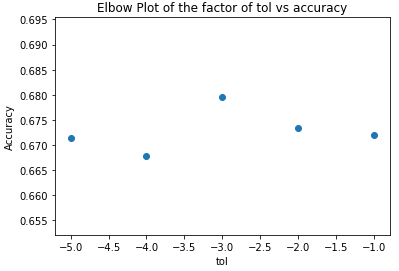
\includegraphics[width=\linewidth]{K_Means_Elbow}
\caption{Elbow plot of the level of convergence of centroids vs accuracy}
\Description{K-Means Elbow Plot}
\end{figure}


\section{Evaluation}

\subsection{Correlations Between Craftables \& Materials}
In general, the craftable BiS equipment correlates very poorly their materials. The Green Lens, a pre-raid BiS head-piece for all magic casting classes, correlates strongest with Heart of the Wild, an extremely common material used for 6 other craftable items. Though the correlation is significant with a p-value of \( 2.84e^{-5} \), a Pearson correlation coefficient of 0.137 and a \( R^2 \) value of 0.0188 show that the correlation is very weak and the SLR model is a poor fit to the data. You can see the emphasis of the lack of correlation in Figure 2 below

\begin{figure}[h]
\centering
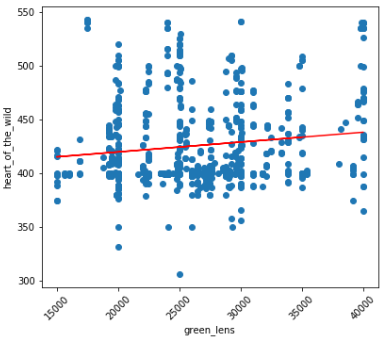
\includegraphics[width=\linewidth]{gl_hotw_corr}
\caption{Correlation and Simple Linear Regression Line of Relationship between minimum buyout price of Green Lens and minimum buyout price of Heart of the Wild.}
\Description{Green Lens and Heart of the Wild Correlation}
\end{figure}

One unique find is the minimum buyout price of Devilsaur Leather shares a very strong correlation with all of craftables it creates. Devilsaur Gauntlets shares a Pearson correlation coefficient of 0.828 with a p-value of 0 and an \( R^2 \) value of 0.68. Devilsaur Leggings also show a significant correlation with Devilsaur Leather, reporting a correlation coefficient of 0.81, a p-value of 0, and an \( R^2 \) value of 0.67. This could be due a combination of the extreme rarity Devilsaur Leather and the low number of items it creates.

\begin{figure}[h]
\centering
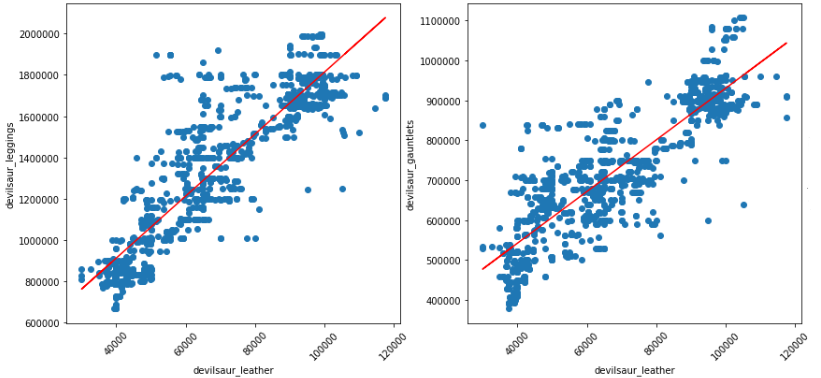
\includegraphics[width=\linewidth]{devilsuar_leather_corr}
\caption{Correlation and Simple Linear Regression Line of Relationship between the minimum buyout price of Devilsaur Leather and minimum buyout price of the items it creates.}
\Description{Devilsaur Leather Correlation}
\end{figure}

Potions and Flasks consistently perform better than BiS equipment in correlating with their main ingredients. All of the high popularity potions share strong, significant correlations with the main required material required to produce them. Greater Fire Protection Potion and Elemental Fire share a correlation coefficient of 0.72, a p-value of 0, and an \( R^2 \) value of 0.52. Free Action Potion, a very power potion for Player-vs-Player PvP content, correlate well with Blackmouth Oil showing a coefficient of 0.780, a p-value of 0, and an \( R^2 \) value of 0.608. Swiftness Potion, a low-level, versatile potion used for PvP, speed-leveling, and raiding, shares a correlation coefficient with Swiftthistle of 0.57, a p-value of 0, and an \( R^2 \) value of 0.327.

\begin{figure}[h]
\centering
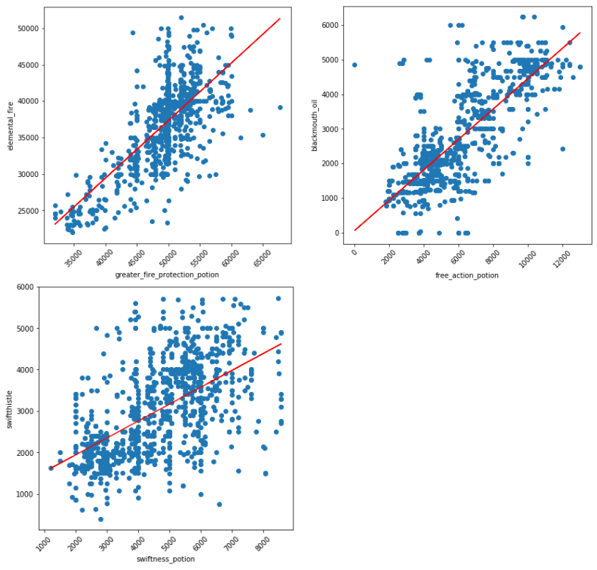
\includegraphics[width=\linewidth]{pot_corr}
\caption{Correlation and Simple Linear Regression Line of Relationship of the minimum buyout price of some of the highest demand potions for end-game content and the main ingredient for crafting the respective potions.}
\Description{Potion Correlation}
\end{figure}

The three flasks observed, Flask of Surpreme Power, Flask of Distilled Wisdom, and Flask of the Titans all share the same main ingredient – Black Lotus. Thus, there are some interesting results from the correlation analysis. The Flask of Surpreme Power shares the strongest correlation with Black Lotus with a correlation coefficient of 0.81 and an \( R^2 \) value of 0.657. Next strongest is Flask of Distilled Wisdom with a correlation coefficient of 0.607 and \( R^2 \) value of 0.369, followed by Flask of the Titans with a correlation coefficient of 0.431 and an \( R^2 \) value of 0.186. All produced a p-value of 0.

\begin{figure}[h]
\centering
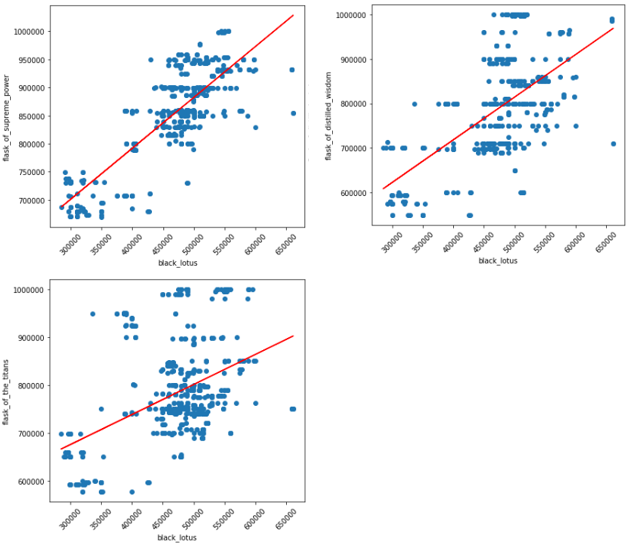
\includegraphics[width=\linewidth]{flask_corr}
\caption{Correlation and Simple Linear Regression Line of Relationship of the minimum buyout price of Black Lotus and the minimum buyout price of the flasks it is used to produce.}
\Description{Flask Correlation}
\end{figure}

\subsection{Time-Series Analysis of Greater Fire Protection Potion}

When splitting the minimum buyout prices of Greater Fire Protection Potion by weekday, the best performing day is Wednesday with a mean price of 4 gold 69 silver 84 copper and the lowest performing day is Tuesday with a mean price of 4 gold 46 silver 94 copper. Though the means were not far off from each other, the spread for Tuesday is much higher with a standard deviation of 95 silver 6 copper compared to Wednesday’s standard deviation of 79 silver 81 copper. Testing the significance of the difference in means with a significance level of \( \alpha = 0.05 \) found a p-value of 0.0102, which is considered significant.

\begin{figure}[h]
  \centering
  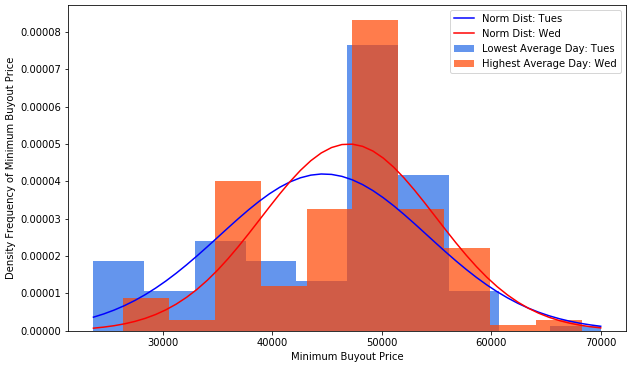
\includegraphics[width=\linewidth]{tues_wed_hist}
  \caption{Normal distibution of the minimum buyout price of Greater Fire Protection Potion between Tuesday (the lowest performing day) and Wednesday (the highest performing day)}
  \Description{Tuesday vs Wednesday Histogram}
\end{figure}

Splitting the minimum buyout prices by hour of the day did not perform as well at splitting them by weekday. The best performing hour is between 9 and 10 PM with a mean price of 4g 84s 10c and a standard deviation of 88s 36c. The worst performing hour is between 4 and 5 PM with a mean of 4g 42s 76c. Though the difference in means is shown to be higher than for splitting the data by day, the spread is significantly higher for both. The p-value of the difference in these means is a 0.271 which is pretty insignificant. These results may have had to do with the small sample size when splitting by hour as opposed to day – 24 intervals instead of 7.

\begin{figure}[h]
  \centering
  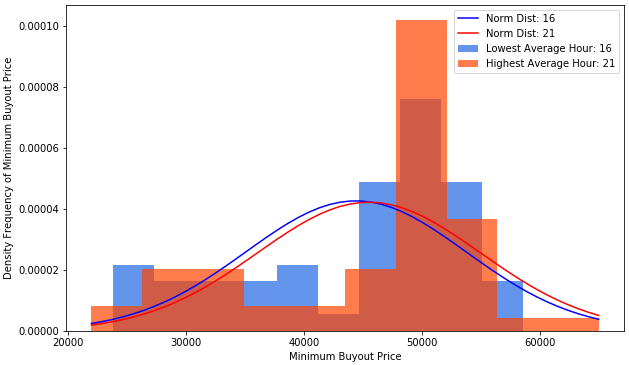
\includegraphics[width=\linewidth]{hourly_hist}
  \caption{Normal distibution of the minimum buyout price of Greater Fire Protection Potion between 4pm (the lowest performing hour) and 9pm (the highest performing hour)}
  \Description{Hourly Histogram}
\end{figure}

Splitting the daily minimum buyout prices by parts of the day (Morning 5am-12pm, Afternoon 12pm-5pm, Evening 5pm-9pm, and Night 9pm-5am) gave much better results than by hour due to the larger sample sizes. Oddly, the difference in means is much smaller with Night having the highest performance at a mean of 4g 71s 98c and a standard deviation of 89s 58c and the Afternoon having the lowest performance at a mean of 4g 50s 17c and a standard deviation of 92s 44c. However, due to the much larger sample sizes the t-test scores a p-value of 0.001, the most significant difference of the three tests.

\begin{figure}[h]
  \centering
  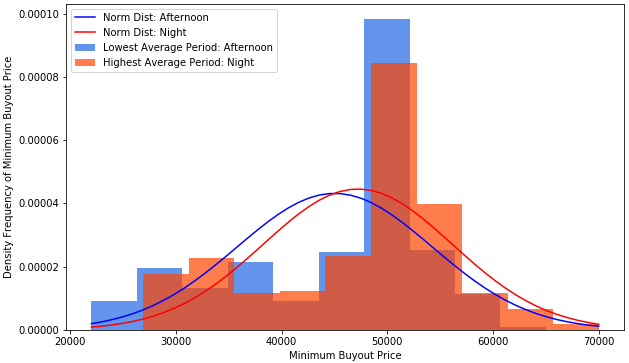
\includegraphics[width=\linewidth]{pod_hist}
  \caption{Normal distibution of the minimum buyout price of Greater Fire Protection Potion between afternoon (the lowest performing part of the day) and night (the highest performing part of the day)}
  \Description{PoD Histogram}
\end{figure}

Using the information from the previous three tests, the data was subset into the theoretical best performing period, a Wednesday night, and the theoretical worst performing period, a Tuesday Afternoon. Wednesday night has a mean price of 5g 1s 26c and a standard deviation of 74s 2c, while Tuesday afternoon has a mean price of 4g 33s 80c and a standard deviation of 90s 60c. The histogram (Figure 9) shows a much more visually noticeable difference between the prices with the Tuesday afternoon low being much lower than the Wednesday night low, and the Wednesday night high being much higher than the Tuesday afternoon high. It is also the only plot where the mode is noticeably higher for Wednesday night than it is for Tuesday afternoon. The p-value for the t-test scored a 1.64e-4, which is extremely significant within any acceptable significance level. Thus, the best time to buy Greater Fire Potion is a Tuesday between 12pm and 5pm and the best time to sell is a Wednesday night between 9pm and 5am.

\begin{figure}[h]
  \centering
  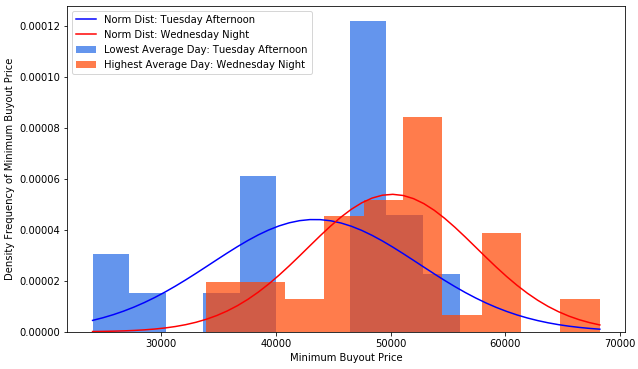
\includegraphics[width=\linewidth]{bestworst_hist}
  \caption{Normal distibution of the minimum buyout price of Greater Fire Protection Potion between Tuesday afternoon (the theoretically worst performing part of the week) and Wesneday night (the theoretically worst performing part of the week)}
  \Description{Worst vs best Histogram}
\end{figure}When splitting the minimum buyout prices of Greater Fire Protection Potion by weekday, the best performing day is Wednesday with a mean price of 4 gold 69 silver 84 copper and the lowest performing day is Tuesday with a mean price of 4 gold 46 silver 94 copper. Though the means are not far off from each other, the spread for Tuesday is much higher with a standard deviation of 95 silver 6 copper compared to Wednesday’s standard deviation of 79 silver 81 copper. Testing the significance of the difference in means with a significance level of \( \alpha = 0.05 \) found a p-value of 0.0102, which is considered significant.

\begin{figure}[h]
\centering
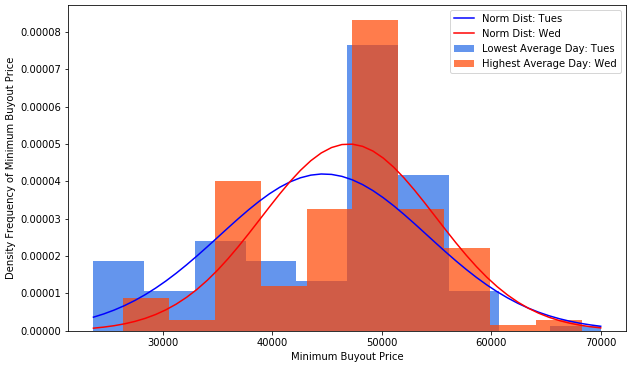
\includegraphics[width=\linewidth]{tues_wed_hist}
\caption{Normal distibution of the minimum buyout price of Greater Fire Protection Potion between Tuesday (the lowest performing day) and Wednesday (the highest performing day)}
\Description{Tuesday vs Wednesday Histogram}
\end{figure}

Splitting the minimum buyout prices by hour of the day does not perform as well at splitting them by weekday. The best performing hour is between 9 and 10 PM with a mean price of 4g 84s 10c and a standard deviation of 88s 36c. The worst performing hour is between 4 and 5 PM with a mean of 4g 42s 76c. Though the difference in means is shown to be higher than for splitting the data by day, the spread is significantly higher for both. The p-value of the difference in these means is a 0.271 which is pretty insignificant. These results may have had to do with the small sample size when splitting by hour as opposed to day – 24 intervals instead of 7.

\begin{figure}[h]
\centering
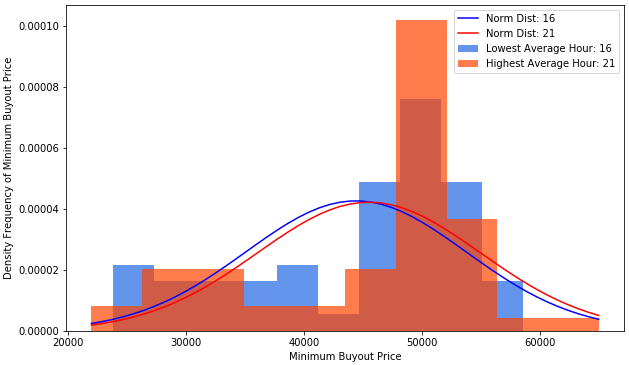
\includegraphics[width=\linewidth]{hourly_hist}
\caption{Normal distibution of the minimum buyout price of Greater Fire Protection Potion between 4pm (the lowest performing hour) and 9pm (the highest performing hour)}
\Description{Hourly Histogram}
\end{figure}

Splitting the daily minimum buyout prices by parts of the day (Morning 5am-12pm, Afternoon 12pm-5pm, Evening 5pm-9pm, and Night 9pm-5am) produces much better results than by hour due to the larger sample sizes. Oddly, the difference in means is much smaller with Night having the highest performance at a mean of 4g 71s 98c and a standard deviation of 89s 58c and the Afternoon having the lowest performance at a mean of 4g 50s 17c and a standard deviation of 92s 44c. However, due to the much larger sample sizes the t-test scores a p-value of 0.001, the most significant difference of the three tests.

\begin{figure}[h]
\centering
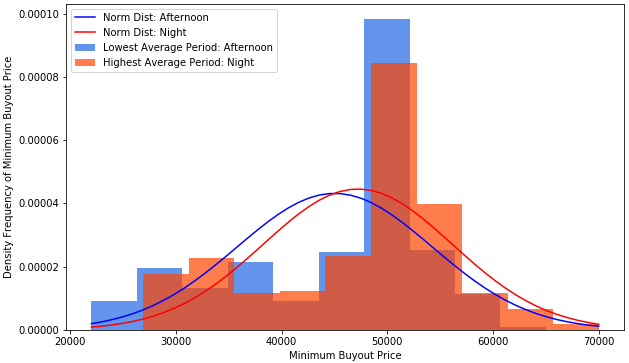
\includegraphics[width=\linewidth]{pod_hist}
\caption{Normal distibution of the minimum buyout price of Greater Fire Protection Potion between afternoon (the lowest performing part of the day) and night (the highest performing part of the day)}
\Description{PoD Histogram}
\end{figure}

Using the information from the previous three tests, the data is subset into the theoretical best performing period, a Wednesday night, and the theoretical worst performing period, a Tuesday Afternoon. Wednesday night has a mean price of 5g 1s 26c and a standard deviation of 74s 2c, while Tuesday afternoon has a mean price of 4g 33s 80c and a standard deviation of 90s 60c. The histogram (Figure 9) shows a much more visually noticeable difference between the prices with the Tuesday afternoon low being much lower than the Wednesday night low, and the Wednesday night high being much higher than the Tuesday afternoon high. It is also the only plot where the mode is noticeably higher for Wednesday night than it is for Tuesday afternoon. The p-value for the t-test scored a 1.64e-4, which is extremely significant within any acceptable significance level. Thus, the best time to buy Greater Fire Potion is a Tuesday between 12pm and 5pm and the best time to sell is a Wednesday night between 9pm and 5am.

\begin{figure}[h]
\centering
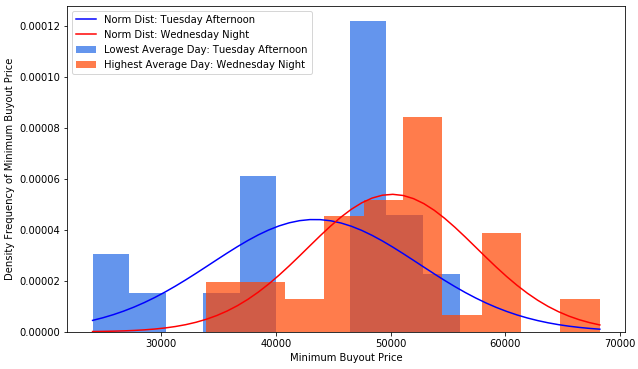
\includegraphics[width=\linewidth]{bestworst_hist}
\caption{Normal distibution of the minimum buyout price of Greater Fire Protection Potion between Tuesday afternoon (the theoretically worst performing part of the week) and Wesneday night (the theoretically worst performing part of the week)}
\Description{Worst vs best Histogram}
\end{figure}


\subsection{K-means Clustering}
Overall, k-means clustering method of classifying the direction of the price change performs horribly. When splitting the price into 3 classes – Decrease in price, increase in price, no price change – the algorithm shows an accuracy of slightly over 30\%. Because the algorithm is only predicting one third of the classes correctly for three classes, it is safe to assume it fails in predicting the price change with any accuracy. In an attempt to increase performance, decreasing price and no change in price are combined into one class and k is decreased to 2. Still, after tuning all parameters to the best performing method, the accuracy only resulted in 70\%. The algorithm has a very high favor towards classifying price changes as decreasing/not changing with 745 predicted correctly and 250 falsely classified as such. Only 76 price changes were correctly classified as increasing, which demonstrates a very poor performance figuring out if a price will increase or not. With the data at-hand, clustering, or binary classification of the price change in general, is not a valid method for predicting the behavior of the minimum buyout price. Because of the randomness and complexity of the auction house, there are too weak of correlations between the variables that may potentially affect price change.

\begin{figure}[h]
\centering
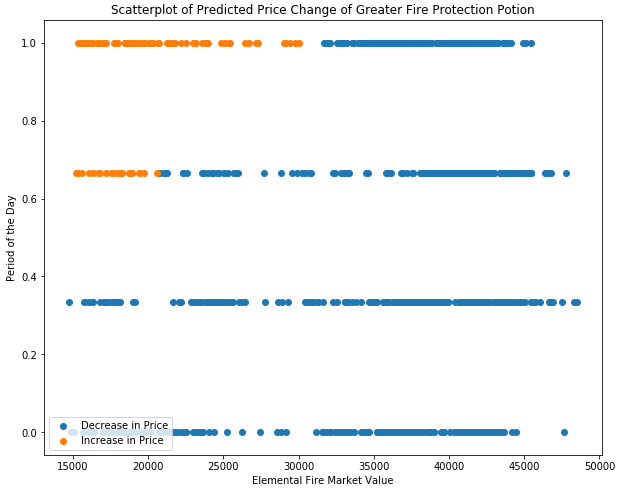
\includegraphics[width=\linewidth]{cluster_plot}
\caption{Scatterplot of the period of the day vs the market value of Elemental Fire split by class determined by k-means clustering algorithm.}
\Description{Cluster Plot}
\end{figure}


\section{Discussion}

\subsection{Correlations Between Craftables \& Materials}
There are a few potential factors that contribute to generally poor correlation with craftable BiS equipment and consumables. The first being that BiS equipment is generally a one-time buy for a player – there is no reason for a player to own more than one of the same helmet or cloak. To the contrary, consumables only have one use per item. This leads to two differences in the buying habits of these item types – consumables are bought significantly more frequently than BiS items and consumables are bought at a higher quantity per purchase compared to BiS items. Similarly, BiS items are bought as an end goal, while consumables are bought to achieve a goal. Because of this, BiS items can be bought at any point in time – a player will buy the item as soon as they have the funds – while consumables follow more of a schedule or routine. Many raiding teams follow a similar raiding schedule due to the scheduled server reset every Tuesday at midnight. Thus, prices of consumables theoretically should be higher earlier in the week and decrease in price as the week ends and most teams have finished their weekly raids. Lastly, BiS caters to a significantly smaller market due to the fact that the “Best in Slot” items are unique for every class. A mage would never buy Devilsaur Gauntlets because there are no stats on the item that are useful for a mage, while rogues entire gameplay mechanics are based around the stats of Devilsaur Gauntlets. Potions such as Greater Fire Protection Potion or Potion of Swiftness are useful, and in some cases required, for all classes to successfully complete content. Thus, a higher population invests in these potions leading to a much higher volatility in price.

Though BiS correlations are generally pretty poor with their items, the relationship between Devilsaur Leather and its BiS craftables is quite high. However, Devilsaur Leather is a unique item compared to other materials. First, it is only used to craft three items, two of which are BiS for the same classes. Devilsaur Gauntlets and Devilsaur Leggings are the BiS for \href{https://www.icy-veins.com/wow-classic/hunter-dps-pve-gear-best-in-slot}{Hunters}, \href{https://www.icy-veins.com/wow-classic/rogue-dps-pve-gear-best-in-slot}{Rogues}, and \href{https://www.icy-veins.com/wow-classic/feral-druid-melee-dps-pve-gear-best-in-slot}{Druids}. \href{https://wowclassicpopulation.com/characters?faction=Alliance&minLevel=60&realm=4647_Grobbulus}{All three classes together make up for 34\% of the World of Warcraft population}, which means there is very high demand for this gear. Devilsaur Leather is also a very high demand item due to its rarity and difficulty to obtain, to the point at which there has been a lot of controversy around farming the item. Some groups on big servers have organized to create a strong-arm on the market, known as \href{https://www.reddit.com/r/classicwow/search/?q=Devilsaur\%20mafia&restrict_sr=1}{Devilaur Mafias}. As a result, Devilsaur Leather and its craftables are a highly volatile market compared to other BiS items.

Potions and Flasks, though used to achieve the same goal and bought in tandem with each other, show slightly different results. Flasks are especially interesting, because all flasks share the same main ingredient – Black Lotus. The ranked correlations between each flask and Black Lotus is proportional to the player population ratio that uses them. Flask of Supreme Power increases spell damage for magic casters and shares the strongest correlation with Black Lotus with a correlation coefficient of 0.811. Damage is also overwhelmingly the most popular role in WoW. 40-man raid teams are generally made up of 3 tanks, 6 to 8 healers, and 29 to 31 damage dealers where 50\% of the damage dealers are magic casters. 5-man dungeon groups are always made up of 1 tank, 1 healer, and 3 damage dealers with generally 2 being magic casters. Flask of supreme power is also used by a large number of popular classes. Mage is tied for the most popular class with Warrior, making up 16\% of the player population. The other classes that may use this item are shadow priests, warlock, and balance druids all of which make up for 46\% of the player population. Though a percentage of these classes may be healers, majority are generally damage dealers. Flask of Distilled Wisdom share the second strongest correlation with Black Lotus with a correlation coefficient of 0.607. It’s ability to increase the caster’s significantly makes it a requirement for healers, as a healer’s main responsibility is their mana management. Healers also make up for the second most popular role for the same reasons stated previously. Flask of the Titans, the required flask for tanks, reports the weakest correlation with Black Lotus with a correlation of 0.431. Tanks are the raid/group leaders, as they control the positioning of the enemy and the direction of the fight. Because of the increased responsibility and difficulty, tanks are the least popular role.


\subsection{Time-Series Analysis of Greater Fire Protection Potion}

The first thing to address is the poor performance of the hourly intervals compared to the other two intervals. Contradictory to the p-value, the difference in sample means between the best performing interval and worst performing interval was much greater than the other two interval groups. This odd behavior and low significance are contributed to by the extremely small data sets compared to the other two methods. The weekday data is split into 7 intervals and the part-of-day data is split into 4 intervals, while the hourly data was split into 24 intervals. If there was more data to sample over a much longer period of time, there would be a chance of a significant difference between the best and worst intervals.

The difference in means between Tuesday Afternoon and Wednesday Night may be attributed to the weekly server schedule of WoW Classic. Even though there is a smaller sample size used than for weekday intervals and part-of-day intervals, this difference results in a p-value of 1.64e-4. In WoW Classic, the week begins on Tuesday after the server reset. Most competitive raid teams schedule their raids for Wednesday and Thursday nights. Because of the increased number of raiders, the price of Greater Fire Protection Potion increases to accommodate the increase in demand. As the week progresses less teams are still completing the raid content and the price drops with the decreased demand. Tuesday afternoon is the last time interval before players begin preparing for the next week’s raiding schedule, and the prices will not recover until that night. Thus, the best time to buy Greater Fire Protection Potions is Tuesday between 12pm and 5pm, and the best time to sell is Wednesday night between 9pm and 5am.

\subsection{K-means Clustering}

It was expected previously to implementing the algorithm for the method to fail. The biggest problem with this method is there is very little correlation between every one predictor variable and the direction in the price change. The first attempt as feature selection uses the differences between the market/historical values and the minimum buyout values. However, this leads to an accuracy of only 53\%. Using the raw values is better, but not ideal with an accuracy of only 70\%. There is also a massive bias toward the price dropping or staying the same – 91\% of the instances are classified to drop. A combination of too many events contributing to price change combined with a high element of randomness makes k-means clustering too simplified of a method to predict price behavior.

\section{Conclusion}

Overall, predicting when to buy or sell solely by comparing the normal distributions of prices in separate time intervals has proven to be the best performing method, while K-means clustering is the worst prediction method. Using confidence interval estimation, it is determined that Tuesday afternoon is the best time to buy Greater Fire Protection Potion and the best time to sell is Wednesday Night with a p-value of 1.64e-4. Though, using clustering only gives an accurate prediction 70\% of the time. It is also shown that building strategies around consumables performs better than using BiS items. The consumables high correlation with their main materials gives the trader a more diverse group of items to trade with their strategy.

\section{Honor Code Pledge}
On my honor, as a University of Colorado Boulder student, I have neither given nor received unauthorized assistance. The University of Colorado Honor Code works by receiving the support and participation of all members in the university community. Such an organization is intended to promote a campus culture that consciously upholds the tenets of academic integrity, and moral and ethical conduct.

\section{Citations and Bibliographies}
\begin{enumerate}
\item u/Mrtyki. “r/Woweconomy - AMA. Made 1000g in 2 Weeks on 1 Character with 10 Gold.” Reddit, Reddit, 11 Oct. 2019, 12:28:44 PM, www.reddit.com/r/woweconomy/comments/dgj6yb/ama\_made\_1000g\_in\_2\_weeks\_on\_1\_character\_with\_10/.
\item Blizzard Entertainment. “Blizzard End User License Agreement.” Blizzard Legal, Blizzard Entertainment, 1 June 2018, www.blizzard.com/en-us/legal/fba4d00f-c7e4-4883-b8b9-1b4500a402ea/blizzardend-user-license-agreement. 
\item Erorus. “Booty Bay Gazette.” Booty Bay Gazette, The Undermine Journal, 9 Oct. 2019, www.bootybaygazette.com/. 
\item Fanbyte. “World of Warcraft.” Wowhead, 2019, classic.wowhead.com/. 
\item Larrikin, CPP. “Monthly Economic Report - April 2019.” EVE Online, CPP, 13 May 2019, www.eveonline.com/article/prg4uv/monthlyeconomic-report-april-2019. 
\item “r/Woweconomy.” Reddit, www.reddit.com/r/woweconomy/. 
\item “r/Classicwow.” Reddit, 2019, www.reddit.com/r/classicwow/.
\item TradeSkillMaster. “Most Advanced Addon for Making Gold in World of Warcraft.” TradeSkillMaster, TradeSkillMaster, 2019, www.tradeskillmaster.com/.
\item “Wow Classic Population - A Census Project.” WowClassicPopulation.com, 2019, wowclassicpopulation.com/.
\item 2017, Icy Veins. “WoW Classic Guides and News.” Icy Veins, 2019, www.icy-veins.com/wow-classic/.

\end{enumerate}

\end{document}
